\section{Finance Simulation}
\label{sec:finance_simulation}
Nike, Salih\\

The finance simulation is connected to almost all other simulations, as costs and profits are ruling an enterprise's daily work. The complete finance graph can be found in appendix [PUT IN APPENDIX PLUS REFERENCE], however, it is part of the overall graph. Just for reasons of clarification and concise structure we developed a separate graph, whereas at least the start node and the leave nodes are exactly the same as in the overall graph. Contrary to the overall graph, we inserted aggregated nodes, that simply sum up the nodes in the overall graphs, so that a clearer overview about how the single financial performance indicators are calculated is possible. Especially for the calculation of the EBIT this graph is important, because it displays all the expenses and all the revenues from different sources neat and clean. A part of the finance graph can be found in figure \ref{fig:financeGraphPart}, which displays the calculation of the net operating profit after tax (NOPAT) and the net worth.

\begin{figure} [!htbp]
    \centering
    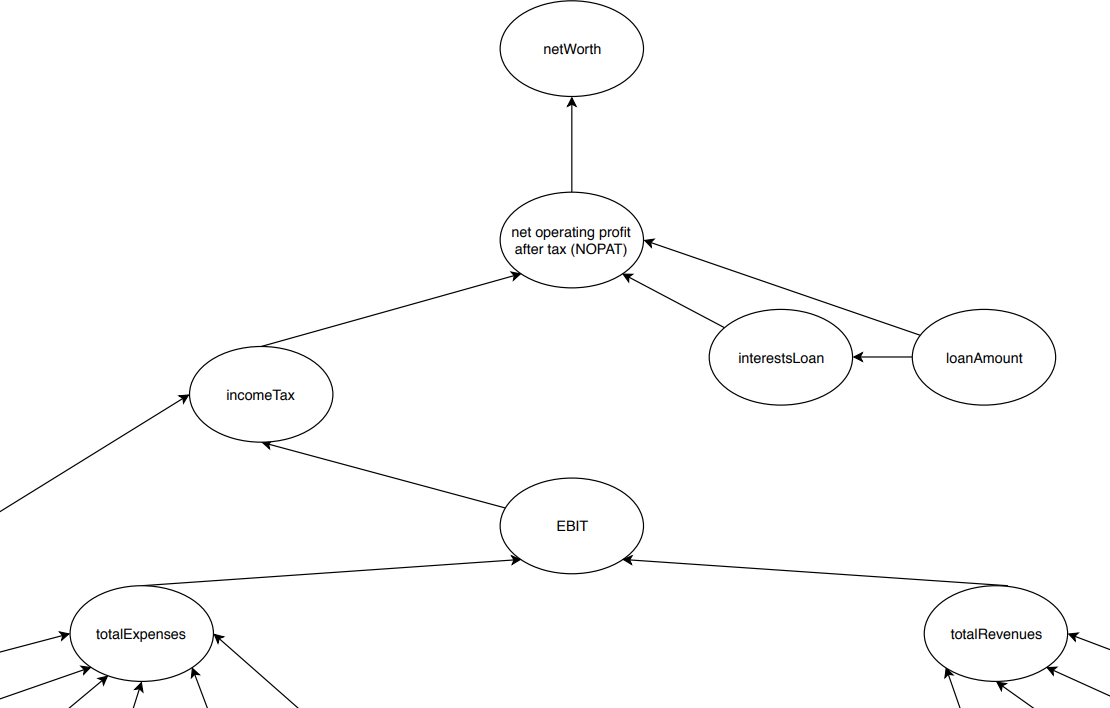
\includegraphics [width=\textwidth] {images/FinanceGraphPart.png}
    \caption{Part of the Finance Graph}
    \label{fig:financeGraphPart}
\end{figure}

The main financial key figure is the company net worth. A company's net worth is the difference between assets and liabilities\footnote{https://www.investopedia.com/terms/n/networth.asp}. In a successful company, this value should be positive and increase continuously. This is adapted from a balance sheet that is usually updated annually. The balance sheet template in table \ref{tab:BalanceSheet} shows an exemplary balance sheet in CapitalismX which is updated monthly for the calculations in the backend. On the assets side there are non-current assets, which include buildings, machinery, vehicle fleets and investments, and current assets, which include components, products, bank and cash. On the liabilities side, the equity capital and the liabilities are shown including loans and total expenses. However, in CapitalismX the company net worth as well as all other financial key figures are calculated in a simplified manner, due to the high complexity in the real world.

\begin{table}[ht]
\label{tab:BalanceSheet}
\begin{tabular}{|p{5.9cm}|p{5.9cm}|}
\hline
\multicolumn{2}{|c|}{\textbf{Balance Sheet}}\\
\hline \textbf{Assets} & \textbf{Liabilities}\\ 
\hline \textbf{I. Non-current assets} & \textbf{I. Equity capital}\\
\hline 1.2 Land and buildings &\\
\hline 1.3 Machines & \textbf{II. Liabilities}\\
\hline 1.4 Vehicle fleet & 2.1 Loans\\
\hline 1.5. Financial investments &  2.2 Total expenses\\
\hline &\\
\hline \textbf{II. Current assets} &\\
\hline 2.1 Components &\\
\hline 2.2 Products &\\
\hline 2.3 Bank and cash &\\
\hline &\\
\hline \textbf{Total Assets} & \textbf{Total Liabilities}\\
\hline
\end{tabular}
\caption{Balance Sheet}
\end{table}

The company’s net worth %@salih: oder der NOPAT???? 
is calculated from the EBIT, that the player has obtained through his or her actions during the game. Added to the EBIT there are the loans a player might have borrowed from the bank, the interest that the player has to expend in order to amortize the loan, and the income tax the player has to pay for all earnings. Accordingly, the net worth is calculated in  function \ref{func:netWorth}.
% @Salih: ist das jetzt noch so korrekt? Weil die Taxes bezahlt er ja täglich, das passt ja also, aber mit den loan interests war das jetzt wie? :o
\begin{equation}
\label{func:netWorth}
    Net~worth = (EBIT~+~\frac{loan~interests}{356})~*~taxPercentage~+~loan~amount
\end{equation}

%$net~worth = (EBITv+loan\ amount+(loan\ interests/365))* taxPercentage$
%Net worth = EBIT + loan amount + (loan interests /360) if day == 01, then Net worth = (EBIT + loan amount + (loan interests / 360) ) * taxPercentage.

The company net worth is an ad hoc calculated key figure, which means that periodically occurring costs, such as interests for loans, that are due on a monthly basis are not included until the beginning of the next month. Resulting from that is a slight decrease of the net worth at the beginning of a month, because at this time the interests for loans are subtracted from the NOPAT.
 
\subsection{Income tax}

In CapitalismX the income tax is levied on a daily basis and can be compared to the income tax paid by a large corporation in the United States of America according to the IAS 12 \textit{Income Taxes} paragraph from the IFRS\footnote{https://www.ifrs.org/-/media/feature/meetings/2018/october/iasb/ap12c-ias12.pdf}, although of course realistically the income tax is levied annually. In order to provide the player a more structured overview about the company’s financial situation, we decided to provide the player with a daily income tax, that is subtracted from the NOPAT, however, for the player it looks like it was subtracted from the net worth. As described in chapter \ref{logistic_simulation} the produced products per day are collected in the warehouse and sent out to the market at the end of the day. Hence, the amount of the income tax varies depending on the quantity of products sold. The income tax percentage can be decreased down to a minimum of 10\% by hiring powerful lobbyists. This process is described in chapter \ref{lobbyist_simulation}.

\subsection{Banking system}

The bank simulation ensures that the player has an additional opportunity to raise capital in case of bottlenecks or for investments. Three types of credit are offered to the player in case of a request. 
The short-term loan requires a repayment within one and twelve months. The interest rate varies between 6\% and 18\%. The medium-term loan is payable within 1-5 years, while the interest rate is between 3\% and 6\%. A long-term loan has a term of more than 10 years and a maximum of 15 years with an interest rate between 1\% and 3\% \footnote{https://www.statista.com/statistics/258174/long-term-interest-rates-worldwide}. 

The bank's credit offers are randomized in the defined intervals to make the game more interesting for the player. Hence, both variables, the duration as well as the interest rates, are randomized on a daily basis. The three types of credit are provided as amortization loans. Thus, the player has a fixed interest rate and a fixed monthly amortization. This reduces the repayment amount over time \footnote{\footnote{https://www.investopedia.com/terms/a/amortized\_loan.asp}}.

However, the raising of capital from the bank is restricted.
The requested loan must not be larger than 30 \% of the company value, which is for reasons of simplification the current company net worth. If this is fulfilled, the player receives three offers with the duration and the interest rate as described above. In the event of a negative check by the bank, so if the requested loan is in fact larger than 30\% of the company value, then the player receives an adjusted offer corresponding to the company value. The new loan amount offered is not greater than 30\% of the company value. The process of the banking simulation is displayed in an activity diagram in figure \ref{jpg:banking}.

\begin{figure}
	\centering
	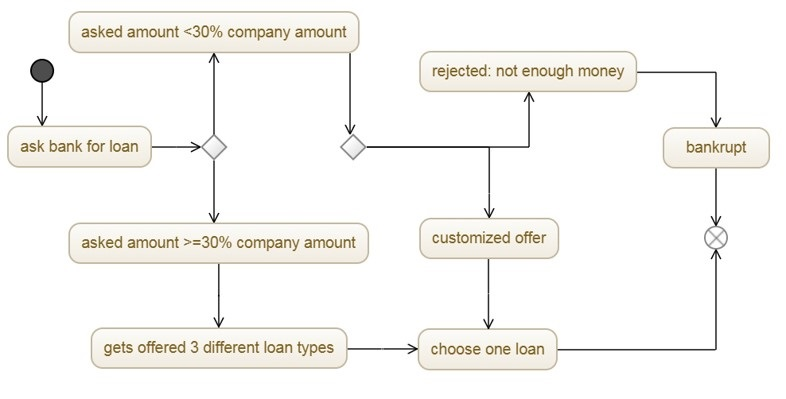
\includegraphics[width=12cm]{images/banking_activity_diagram.jpg}
	\caption{Activity Diagram Banking Simulation}
	\label{jpg:banking}
\end{figure}

The following variables and formulas are defined for the calculation of the repayment, but also for the observation of the bank restrictions.

\begin{itemize}
    \item variables:
    \item Principal of Loan = S; retirement= a; term= t; interest rate= i; principal balance per year= S\textsubscript{n}; Rate= r. 
    \item formulas:
 $$a={\dfrac{S}{t}}$$
 $$S_n=S-(a*t)$$
 $$Interest\ rate\ per\ year: i_n=S_t*i $$
 $$Rate\ per\ year: r_t=a+i_t$$
$$Rate\ per\ month:r_m= {\dfrac{r_t}{12}} $$
    
\end{itemize}

The Bank observation in CapitalismX is regulated as follows:
\begin{equation}
\begin{aligned}
    If (loan * 30\% ) \geq  \text{net worth} \xrightarrow{} \text{accepted} \ \text{(offer three credit forms)} \\
    If (loan * 30\%) < \text{net worth} \xrightarrow{} \text{reject AND offer} \ (net worth / 30\%)
\end{aligned}    
\end{equation}


\subsection{EBIT calcuation}

The next level under the company's NOPAT is the EBIT, which are the earnings before interest and tax, a commonly used key financial indicator in company's financial statements. \cite{lee_e_2006} Again, the calculation of the EBIT is simplified for the business simulation game at hand. To sum it up, all revenues are added to the EBIT whereas the total expenses are subtracted. The EBIT is displayed in the cashflow section of the finance view and updated on a daily basis.

\subsubsection{Revenues}
In order to calculate the EBIT, it is necessary to first consolidate all the revenues. The total revenue is calculated by adding all incoming cash flows, which are:
\begin{itemize}
    \item Goods sold, displayed by the total sales of products, which can be derived by multiplying a product’s price, which is set by the user with the amount of units sold. %vllt noch den Begriff aus dem full graph (ProductSale (PS) mit sales figures und so) eingehen?
    \begin{equation}
        Sales: S(P) = \sum price\index{Product} * units~sold
    \end{equation}
    Goods sold is an aggregated value from the product sale, which is calculated in chapter [CHAPTER REFERENCE].
    \item Equipment sold. The player has the possibility to sell used machinery or vehicles, that he or she does not need anymore. The calculation for the residual value is based on a straight line depreciation:
     \begin{equation}
     Annual \ depreciation = {\dfrac{cost \ of \ the \ asset}{useful \ life \ of \ the \ asset}}
    \end{equation}
     \begin{equation}
     residual \ value = {{cost \ of \ the \ asset} - {annual \ depreciation * t }}    
     \end{equation}
    
    \item Land and buildings sold, which are calculated similar to the equipment sold. %more info needed!!! As above
  
    \item Investments, which are either positive or negative incomes from the investment area in the financial dashboard. %more info needed!!!
\end{itemize}

To put it into a nutshell, the total revenues can be calculated according to the formula \ref{func:totalRevenue}:

\begin{equation}
\label{func:totalRevenue}
\begin{split}
    total \ revenue = \sum goods \ sold \ + \ machinery \ sold \ + \\\ vehicles \ sold \  + \ buildings \ sold \ + \ investments   
\end{split}
\end{equation}

\subsubsection{Expenses}
The other part needed to calculate the EBIT are the total expenses. All costs and expenditures that occur across all other simulations are accounted as expenses. The total expenses consist of:
\begin{itemize}
    \item Total HR costs from the HR simulation, which is the sum of all salaries and the aggregated sum of all trainings and courses for employees. 
    \begin{equation}
        Total~HR~costs = \sum salary_{employee} + training \ and \ courses_{cost}
    \end{equation}
    The salaries, which are viewed as costs from the finance perspective, vary depending on the employees. The calculation of these costs can be found in chapter  \ref{sec:HRsim}.
    \item Warehousing costs, which is the sum of the acquisition costs % or sth like aquisition costs and depreciation displayed for a daily value???
    for all warehouses, the monthly costs for warehouses \textit{cWH} (cf. equation \ref{func:cWH}) and the daily storage costs \textit{sC} (cf. equation \ref{func:SC}). All produced goods are collected at a warehouse and sent out to the market at the end of the day but they do not cause storing costs. Only when producing more products than the market currently demands the spare products are stored in a warehouse, which causes warehousing and storage costs. Added to that, the components which are not manufactured into products yet generate warehousing costs, as they need to be stored until ready for production. The calculation of the storing and the acquisition costs can be found in chapter \ref{warehouse_simulation}. 
    \item Logistic costs, which occur inevitably when selling or retailing goods. The total logistic costs depend on the type of logistics chosen by the player. There are two possibilities: sending packages with an own internal fleet or by hiring an external logistic partner. The total logistic costs can be calculated as follows:
    \begin{equation}
        Total \ logistic \ costs = \sum tTC + tIDC + tCCLP + tEDC
    \end{equation}
    The exact calculation of these costs can be found in chapter \ref{logistic_simulation} and is also visualized in the full finance graph [REFERENCE APPENDIX].
    \item Production costs, which occur when manufacturing components to products. The calculation of these costs can be found in chapter \ref{sec:productionSim}. The total production costs is the sum of variable and fixed production costs. The variable costs are 
    \begin{equation}
        Variable \ costs = \sum tCC + eco \ costs
    \end{equation}
    whereas the calculation of the \textit{tCC} and \textit{eco costs} can be found in chapters \ref{procuresim} and \ref{sec:compEco-idex}. The fixed costs in production are aggregated from facility rent, electricity, purchased asset costs and machinery depreciation costs
    \begin{equation}
    \begin{split}
        Fixed \ costs = \sum facility \ rent + electricity + purchased \ \\ asset \ costs \ + machinery \ depreciation \ costs
    \end{split}
    \end{equation}
    \item Marketing costs, which occur when starting marketing activities like marketing campaigns, market research or press releases (cf. chapter \ref{market_research_simulation}). The total marketing costs also include all costs that are derived from activities to improve the company image, such as hiring a management consultant, donating for social engagements, or promoting a green company image. These costs can be found in chapter \ref{company_image}. Also, hiring a lobbyist for political reasons or to decrease the tax percentage, belongs to the total marketing costs. The calculation of these costs can be found in chapter \ref{lobbyist_simulation}. Accordingly, the total marketing costs are aggregated as follows:
    \begin{equation}
    \begin{split}
        Total \ marketing \ costs = \sum lobbyist_{price} \ + \ campaign_{price} \\\ + \ marketResearch_{price} \ + \  managementConsultancy_{price}
    \end{split}
    \end{equation}
    \item Support costs, which occur if the player chooses to offer product support and maintenance for customers. The total support costs \textit{tSC} calculation can be found in chapter \ref{product_support_simulation}.
\end{itemize}

According to the list of total revenues and total eepenses above, the EBIT can be calculated as follows in function \ref{func:ebit1}. This equation is illustrated by the total finance graph, which can be found in the appendix [REFERENCE]. 
\begin{equation}
\label{func:ebit1}
    EBIT = total~revenues - total~expenses
\end{equation}
whereas total revenues are calculated as in function \ref{func:totalRevenue}, and total expenses are calculated as in the following function \ref{func:ebit2}
\begin{equation}
    \label{func:ebit2}
    \begin{split}
       Total \ expenses = \sum total \ HR \ Costs + total \ Warehousing \ Costs \\\ +  total \ Logistics \ Costs + total \ Production \ Costs \\\ + total \ Marketing \ Costs + total \ Support \ Costs 
    \end{split}
\end{equation}


\subsection{The Finance Dashboard}
Describe UI – what is behind the Finance dashboard? E.g. cashflow – all values mentioned above on a quarterly basis, net worth on a daily basis, etc. - SALIH

Financing from within the business is the internal financing, while financing from organizations outside the company is called external financing. Equity financing occurs, when raising money in exchange for a share of ownership in the business whereas borrowing money, that must be repaid over a period of time, is the debt financing. 
In CapX the player has 3 financing options at his disposal. Due to the high complexity financing options such as leasing, factoring, increase of deposits or provisions were not conceptualized. 
The simplest and most common financing in CapX is the sale of products whose profits can be used for new investments. The linear depreciation of machines, trucks and buildings has the advantage that one thing can be converted into CapCoins at the remaining value at the click of a mouse \footnote{https://www.modu-learn.de/verstehen/finanzen/finanzierungsarten/}.
In the event that internal financing is no longer feasible, it is possible to borrow money from the bank. These three financing options are explained in more detail below.

– SALIH
Describe how implemented in prototype: net worth of company equals profit, taxes are not considered - profit equals ebit, so interests and taxes are substracted to get net worth - [should be done, after final implementation]

Note: networth updated daily. cashflow the left three values are stable per quartal, but the right column in the cashflow is updated daily, as it is more convenient for the player.